%%%%%%%%%%%%%%%%%%%%%%%%%%%%%%%%%%%%%%%%%%%%%%%%%%%%%%%%%%%%%%%%%%%%%%%%%%%%%%%%%%%%%%%%%%%%%%%
%% Description:       Programmentwurf advanced software engineering
%% Author:      Manuel Berg, m.berg@enbw.com
%%  -*- coding: utf-8 -*-
%%%%%%%%%%%%%%%%%%%%%%%%%%%%%%%%%%%%%%%%%%%%%%%%%%%%%%%%%%%%%%%%%%%%%%%%%%%%%%%%%%%%%%%%%%%%%%%

\titlespacing*{\chapter}{0pt}{-30mm}{10pt}
\titleformat{\chapter}[display]
  {\normalfont\bfseries}{}{10pt}{\Huge\thechapter.\quad}
  
\chapter{Weitere Prinzipien (8P)}
\pagestyle{scrheadings}
\clearscrheadfoot
\pagenumbering{arabic}
\setcounter{page}{4}
\ofoot[\pagemark]{\pagemark}
%\ohead[\headmark]{\headmark}
\onehalfspacing

\section{Analyse GRASP: Geringe Kopplung (4P)}
\emph{[jeweils eine bis jetzt noch nicht behandelte Klasse als positives und negatives Beispiel geringer
Kopplung; jeweils UML Diagramm mit zusammenspielenden Klassen, Aufgabenbeschreibung der
Klasse und Begründung warum hier eine geringe Kopplung vorliegt bzw. Beschreibung, wie die
Kopplung aufgelöst werden kann]}

\subsubsection{Positiv-Beispiel}
\noindent Eine geringe Kopplung wurde durch den Einsatz des Observer-Patterns zwischen der für die Visualisierung zuständigen \enquote{GameFrame}-Klasse und der für den Spielablauf zuständigen \enquote{GameService}- Klasse erreicht. Das heißt, wenn in der UI durch den Benutzer eine Aktion ausgeführt wird, wird die \enquote{GameService}-Klasse benachrichtigt. Bei der Benachrichtigung weiß das benachrichtigende Objekt nichts Näheres über das zu benachrichtigende Objekt. Anders ausgedrückt, das Observable kennt nur die Observer-Schnittstelle. Dadurch wurde hier eine lose Kopplung geschaffen. 

\begin{figure}[htbp]
\centering
\centerline{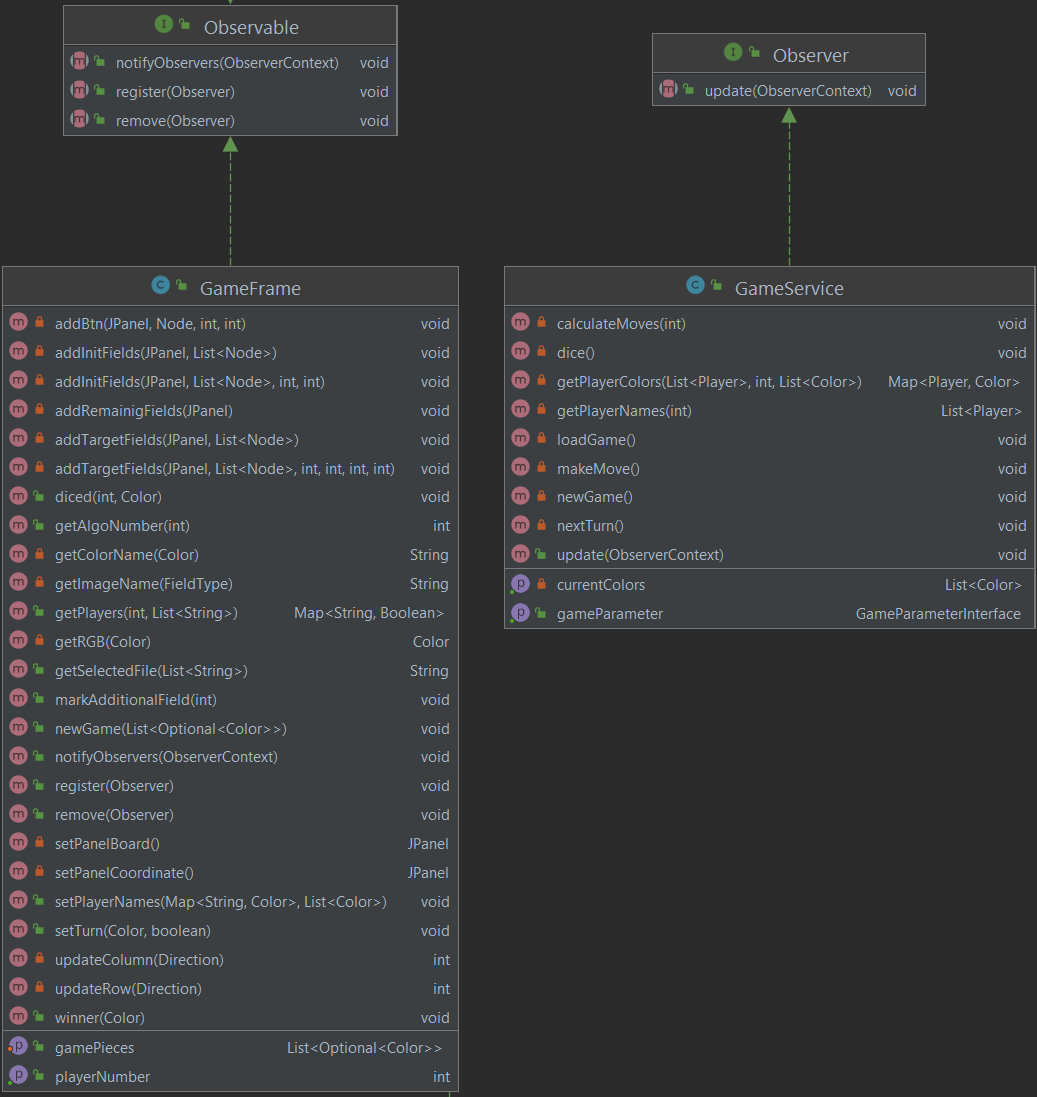
\includegraphics[scale=1]{grasp1}}
\caption{Positiv-Beispiel GRASP [Eigene Darstellung aus \emph{IntelliJ}]}
\label{fig:grasp1}
\end{figure}

\newpage
\subsubsection{Negativ-Beispiel}
\noindent Eine starke Kopplung liegt zwischen der \enquote{Algorithm}- Klasse und der \enquote{AbstractControl\-Mechnism}-Klasse vor. Erstere berechnet einen Zug, der nicht durch einen Benutzer ausgeführt wird -- wenn also ein Benutzer gegen den Algorithmus spielt. Die \enquote{AbstractControl\-Mechnism}-Klasse ruft die Zugberechnung auf. Die Klasse ist abstrakt, da der Aufruf für ein 4-Personen- oder ein 6-Personen-Spielfeld gleichermaßen gilt. 

Eine starke Kopplung liegt vor, da hier auf die konkrete \enquote{Algorithm}- Klasse zuge\-griffen wird. Die Kopplung könnte man durch die Implementierung einer Algorithm-Schnittstelle lockern. Dadurch könnten auch verschiedene Algorithmen implementiert werden.

\begin{figure}[htbp]
\centering
\centerline{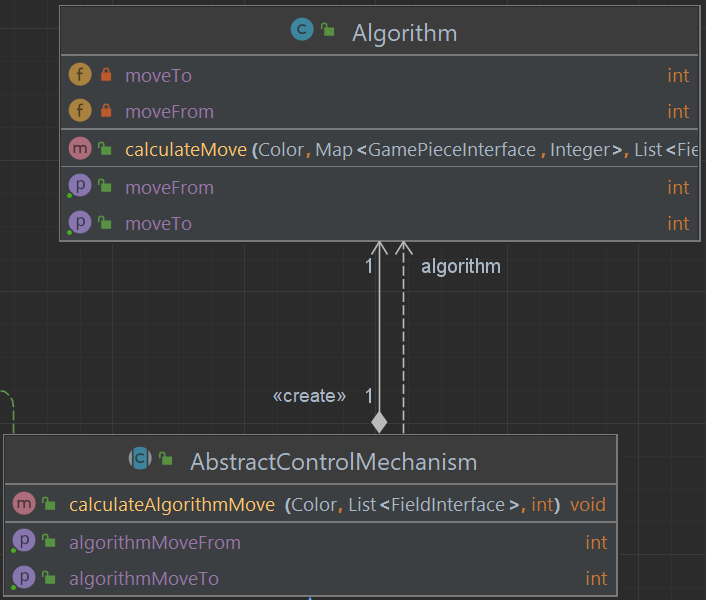
\includegraphics[scale=.6]{grasp2}}
\caption{Negativ-Beispiel GRASP [Eigene Darstellung aus \emph{IntelliJ}]}
\label{fig:grasp2}
\end{figure}

\newpage
\section{Analyse GRASP: Hohe Kohäsion (2P)}
\emph{[eine Klasse als positives Beispiel hoher Kohäsion; UML Diagramm und Begründung, warum die
Kohäsion hoch ist]}

\noindent Die Kohäsion erhöht sich, je mehr Verantwortlichkeiten und Teilaufgaben in andere Klassen ausgelagert sind. Ein Beispiel für hohe Kohäsion wäre hier der dem Spielfeld unterliegende Graph.

\todo{Bild}

\noindent In der \enquote{Graph}-Klasse wird der Graph aufgebaut. Hierzu wurden aber nicht alle Verantwortlichkeiten in dieser Klasse belassen, sondern in vier weitere Klassen ausgelagert.

\begin{itemize}
    \item Die \enquote{Node}-Klasse stellt einen Knoten dar und enthält den Feldtyp (Siehe \enquote{FieldType}) dieses Knotens und die ausgehenden Kanten (Siehe \enquote{Edge})
    \item Das \enquote{FieldType}-Enum gibt den Feldtyp an. Das kann ein neutrales Feld sein oder zum Beispiel ein rotes Startfeld oder ein gelbes Zielfeld.
    \item Die \enquote{Edge}-Klasse enthält den Zielknoten, die Richtung (Siehe \enquote{Direction}) und die Information, ob es ein Default-Kante ist. Letzteres bedeutet, dass die Kante von allen Spielfiguren befahren werden kann. Dies ist zum Beispiel bei der Kante zu den Zielfeldern der jeweiligen Farben nicht der Fall.
    \item Das \enquote{Direction}-Enum gibt an, in welche Richtung die Kante geht.
\end{itemize}

\newpage
\section{DRY (2P)}
\emph{[ein Commit angeben, bei dem duplizierter Code/duplizierte Logik aufgelöst wurde; Code-Beispiele
(vorher/nachher); begründen und Auswirkung beschreiben]}

\noindent Die Klasse \enquote{GraphUtilities} wurde hinzugefügt, da die jetzt enthaltenen vier Methoden früher von den drei Klassen \enquote{Graph}, \enquote{AbstractBoard} und \enquote{ControlMechanismFour} jeweils extra implementiert wurden und sich der Code dadurch dupliziert hat. Das Ergebnis:

\begin{figure}[htbp]
\centering
\centerline{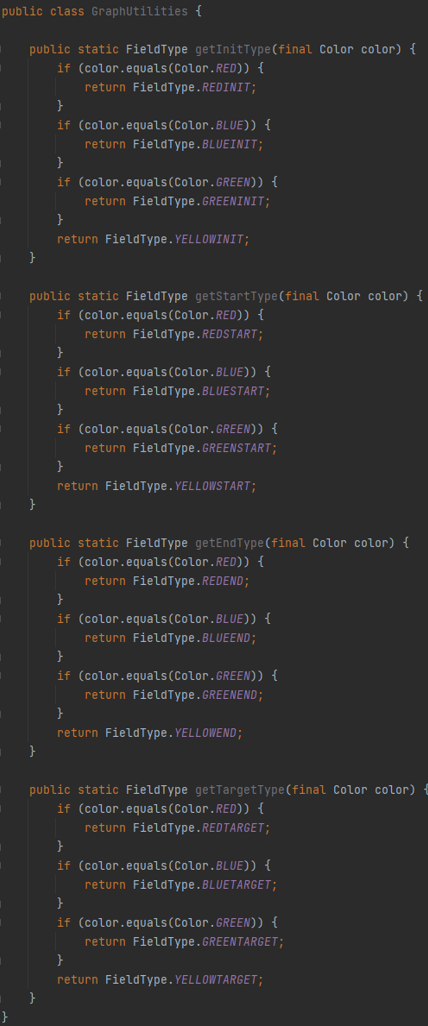
\includegraphics[scale=.6]{dry1}}
\caption{DRY [Eigene Darstellung aus \emph{IntelliJ}]}
\label{fig:dry1}
\end{figure}

\noindent In der \enquote{Graph}-Klasse waren früher alle vier Methoden, in der \enquote{AbstractBoard}-Klasse war nur die \enquote{getInitType}-Methode und in der \enquote{ControlMechanismFour}-Klasse waren ebenfalls alle vier Methoden vorhanden. Der Unterschied zum jetzigen Stand besteht darin, dass die Methoden mittlerweile statisch gemacht worden sind. Da sich innerhalb der Methode nichts verändert hat, sei hier der frühere Stand nicht als Codebeispiel aufgezeigt.

Positiv ist, dass sich der Code durch das Eliminieren von Duplikaten reduziert hat. Außerdem ist aus den einzelnen Klassen Code, der nicht zu deren Verantwortlichkeiten gezählt hat, herausgenommen worden. 

Die Klasse \enquote{GraphUtilities} existierte bis zu dem Commit \enquote{\texttt{Removed duplicated code to GraphUtilities}}.